\documentclass[12pt,a4paper]{article}
\usepackage[utf8]{inputenc} % sempre salve seus arquivos como UTF8
\usepackage[T1]{fontenc}
\usepackage[english]{babel}

\usepackage[left=2.5cm,right=2cm,top=2cm,bottom=2.5cm]{geometry}
\usepackage{amsmath}
\usepackage{amsthm}
\usepackage{amsfonts}
\usepackage{graphicx}
\usepackage{algorithm}
\usepackage{color}
\usepackage[noend]{algpseudocode}
\usepackage{mathtools}
\usepackage{subfig}

% load times font
\usepackage{mathptmx}
\usepackage[scaled=.90]{helvet}
\usepackage{courier}

% comandos
\newcommand{\mdc}[1]{\mathrm{mdc}(#1)}

\DeclarePairedDelimiter\ceil{\lceil}{\rceil}
\DeclarePairedDelimiter\floor{\lfloor}{\rfloor}

% Foot without marker
\newcommand\blfootnote[1]{%
	\begingroup
	\renewcommand\thefootnote{}\footnote{#1}%
	\addtocounter{footnote}{-1}%
	\endgroup
}

\title{MO446 -- Introduction to Computer Vision  \\ Project 0}
\author{Breno Leite  \\ Guilherme Leite}
\date{10/08/2017}

\begin{document}

\maketitle
\blfootnote{\textit{\textbf{Important note:} The borders seen in the figures are not part of the image, they are figurative information about the starting and ending points of the image. Moreover, all the image scales in this report were changed in order to make the text more readable.}} \\

%% ---------------- Starts here --------------------------------

\textbf{Question 1 - Input images} \\

The Figure \ref{fig:p0-1-0} was used as an input to all the exercises, as specified it is a colored image, rectangular and its type is \emph{PNG}. The image dimensions are 400x300, which satisfies the required size. \\

\begin{figure}[!h]
	\centering
	{%
		\setlength{\fboxsep}{1pt}%
		\setlength{\fboxrule}{1pt}%
		\fbox{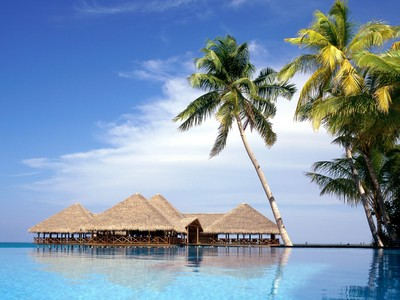
\includegraphics[scale=0.8]{input/p0-1-0}}%
	}%
	\caption{Input image used in the questions (\textbf{p0-1-0})}
	\label{fig:p0-1-0}
\end{figure}

\textit{Note:} The image was converted from \emph{JPG} to \emph{PNG} format. 

\newpage


\textbf{Question 2 - Color planes} \\

\textbf{2-a) } A PNG image is represented in RGB format, which means that there are three channels for each pixel. These channels represents the intensity of each color, in a determined pixel, RGB stands for: Red, Green, and Blue. The Figure \ref{fig:p0-2-a-0} represents an image obtained by swapping the red and blue channel in the input image.

\begin{figure}[!h]
	\centering
	{%
		\setlength{\fboxsep}{1pt}%
		\setlength{\fboxrule}{1pt}%
		\fbox{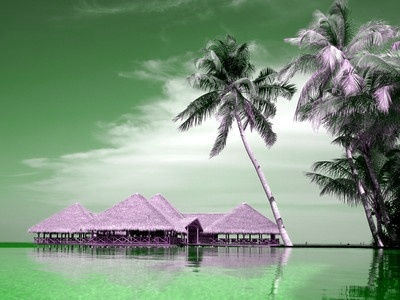
\includegraphics[scale=0.8]{output/p0-2-a-0}}%
	}%
	\caption{Input image with red and blue channels swapped (\textbf{p0-2-a-0})}
	\label{fig:p0-2-a-0}
\end{figure}

We can note a heavy intensity of green in the image after the swap, the reason for that is explained looking at the original image. Most of the pixels in the original image has a low intensity of red, in opposite, the intensity of blue is quite high mainly because of the water and sky. When the swap occurs, all the blue intensity goes to red highlighting things that had a little bit of red intensity on the original image, like the fences. \\

In other hand, all the intensity from the red (really low on the original image) goes to blue. So, that makes the intensity of blue goes down in places that blue was too high (e.g. water and sky). This way, the green color becomes more intense on places that blue was predominant on the original image, explaining the green lake.\\

\newpage

\textbf{2-b) } A monochrome or grayscale images is composed by a single channel, which ranges from 0 to 255 as RGB channels. Thus, create a monochrome image from the green channel is a straightforward procedure, it is just a copy of the green channel into a new image. The result obtained using this procedure on the input image is seen on image (\textbf{p0-2-b-0}).

\begin{figure}[!h]
	\centering
	{%
		\setlength{\fboxsep}{1pt}%
		\setlength{\fboxrule}{1pt}%
		\fbox{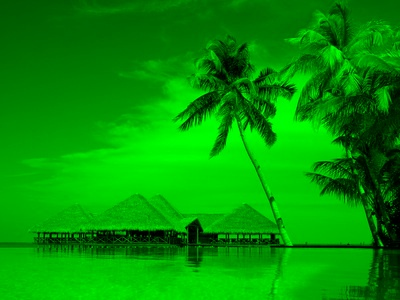
\includegraphics[scale=0.7]{output/p0-2-b-0}}%
	}%
	\caption{Monochrome image created from green channel (\textbf{p0-2-b-0})}
	\label{fig:img-green}
\end{figure}

As shown in the figure, the representation of the image stills really good. The reason for this is the high intensity of the green channel in the original image, which makes this channels, by its own, a good representation for image.\\

\textbf{2-c) } Using the same structure as in \textbf{2-c}, we this time use the red channel to create the new monochrome image, which is shown on image (\textbf{p0-2-c-0}).

\begin{figure}[!h]
	\centering
	{%
		\setlength{\fboxsep}{1pt}%
		\setlength{\fboxrule}{1pt}%
		\fbox{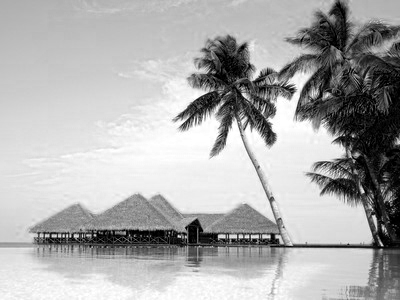
\includegraphics[scale=0.7]{output/p0-2-c-0}}%
	}%
	\caption{Monochrome image created from red channel (\textbf{p0-2-c-0})}
	\label{fig:img-red}
\end{figure}

In this image, we are able to see more blurred areas. The reason for this result is the low intensity of the red channel over the image pixels, which makes just the channel red not as good representation as the green channel.

\textbf{2-d) } The image created from the green channel (\textbf{p0-2-b-0}) looks more like what we expected, this is explained by three channels of the image. As said before, the original image is more intense on the green channel than in the red channel\footnote{Mean values for each channel in the original image: Red: 127.40, Green: 149.85, Blue: 173.02}. We normally would expect that the green approach better express the image, mainly because the nature of the green color in the real world. However, we can not expect this result for every image. \\

In contrast, we would expect a computer to work better in an image extracted from the red channel, the intuition is that the color red gives a better contrast to the image. In this way, the information like shapes of objects on the image are highlighted in the monochrome image, one example is the contrast between the sky and the clouds on image (\textbf{p0-2-c-0}). \\

\textbf{Question 3 - Replacements of pixels} \\

In this question we merge the results shown on image (\textbf{p0-2-b-0}) and image (\textbf{p0-2-c-0}). In order to do that, we inserted the centered 100x100 pixels from image \textbf{p0-2-b-0} into the image \textbf{p0-2-c-0}, the result is shown on image \textbf{(p0-3-0)}. 


\begin{figure}[!h]
	\centering
	{%
		\setlength{\fboxsep}{1pt}%
		\setlength{\fboxrule}{1pt}%
		\fbox{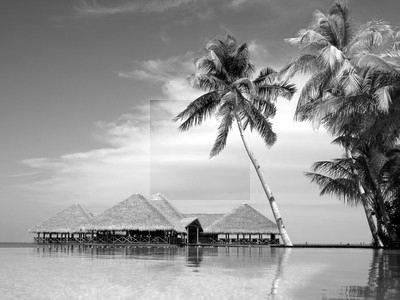
\includegraphics[scale=0.5]{output/p0-3-0}}%
	}%
	\caption{Pixels centered (100x100) from Figure \ref{fig:img-green} into Figure \ref{fig:img-red} (\textbf{p0-3-0})}
	\label{fig:p0-3-0}
\end{figure}

After that, we inserted the generated image (\textbf{p0-3-0}) into its respective channel (green) in the original image. The result is shown on image (\textbf{p0-3-1}).

\begin{figure}[!h]
	\centering
	{%
		\setlength{\fboxsep}{1pt}%
		\setlength{\fboxrule}{1pt}%
		\fbox{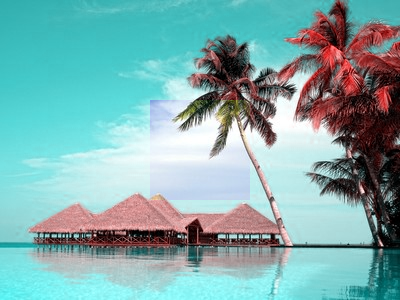
\includegraphics[scale=0.6]{output/p0-3-1}}%
	}%
	\caption{Original image with green channel replaced from Figure \ref{fig:p0-3-0} (\textbf{p0-3-1})}
	\label{fig:p0-3-1}
\end{figure}

As we can see, the image is almost the same as the original input, except by the center part. If we recall, image (\textbf{p0-2-b-0}) is formed by two different images. And, each of them are monochrome images created from the green and red channels of the original input. Figure \ref{fig:channels} shows how the channels representations is represented on image (\textbf{p0-3-1}), which was created by the insertion. \\

\begin{figure}[!h]
	\centering
	{%
		\setlength{\fboxsep}{1pt}%
		\setlength{\fboxrule}{1pt}%
		\fbox{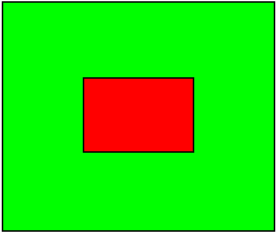
\includegraphics[scale=0.5]{report/image-color}}%
	}%
	\caption{Channels representation layout in the Figure \ref{fig:p0-3-0}}
	\label{fig:channels}
\end{figure}

When we replace image \textbf{p0-3-0} inside the green channel of the original input, all the pixels outsize the box at the center are equal, which keeps the same pixels for all the outside-box part. In contrast, the pixels inside the box, which represents the red color, overwrites the green pixels in that region forming a different image. \\


\textbf{Question 4 - Arithmetic and geometric operations} \\

\textbf{4-a) } The minimum and maximum values from the image \textbf{p0-2-b-0} (\emph{img-green}) are 0 and 255, respectively. The mean value is 149,85 and the deviation is 57,94. The computation for all these values were made using the python library \emph{numpy}, which is a library design for scientific computing. \\

All these function are already implemented into the \emph{numpy} library, so, instead of code snippets we will be showing the function names and the basis formulas that each function is implemented. The functions \emph{numpy.min()} and  \emph{numpy.max()} find the highest and lowest element in a given array, this procedure implemented by \emph{numpy} is pretty straightforward, so we will not show any formulas. \\

Moreover, in order to obtain the mean, we used the \emph{numpy.mean()} that returns the average value given an array. This function implements the following formula: 

$$\bar X = \frac{\sum_{1}^{n} X_i}{N}$$

where $X_i$ is each pixel in the image and $N$ is the total number of pixels in the image. The standard deviation is implemented by the function called \emph{numpy.std()}, this function is based in the following equation:
$$ S = \frac{\sqrt[]{\sum {(x_i - \bar{x})^2}}}{N} $$

In which, $X_i$ is each pixel in the image, $\bar X$ is the mean value and $N$ is the total number of pixels in the image.

\newpage

\textbf{4-b) } In this question the image \textbf{p0-2-b-0} (\emph{image-green}) was used, we subtracted the mean value from all of the pixels, divided them by the standard deviation, multiplied them by 10 and added back the mean value. Figure \ref{fig:p0-4-b-0} is the output image after these operations.


\begin{figure}[!h]
	\centering
	{%
		\setlength{\fboxsep}{1pt}%
		\setlength{\fboxrule}{1pt}%
		\fbox{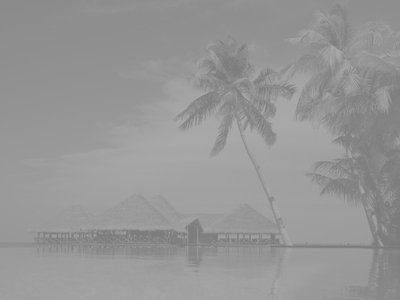
\includegraphics[scale=0.7]{output/p0-4-b-0}}%
	}%
	\caption{Normalized image from image-green (\textbf{p0-4-b-0})}
	\label{fig:p0-4-b-0}
\end{figure}

The image lost a great portion of it's contrast, which could help removing noise from the image or maybe adjust the overall contrast of it. The idea behind it is that, the operations applied reduces the presence of pixels with values too far apart from the others, meaning, pixels that diverge too much are normalized within a certain range of values. \\


\textbf{4-c) } The image \textbf{p0-2-b-0} was also used in this question, so, we shifted twice all pixels to their left. In here, we could either fill the new values in the right size with zero, or we could move the shifted-off part to the right part of the image. The first one was selected because of simplicity to work. The Figure \ref{fig:p0-4-c-0} shows the result image after the shift.

\begin{figure}[!h]
	\centering
	{%
		\setlength{\fboxsep}{1pt}%
		\setlength{\fboxrule}{1pt}%
		\fbox{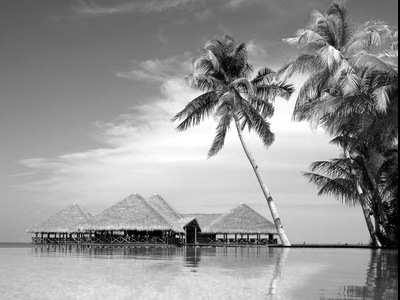
\includegraphics[scale=0.7]{output/p0-4-c-0}}%
	}%
	\caption{2 pixels shifted image from image-green (\textbf{p0-4-c-0})}
	\label{fig:p0-4-c-0}
\end{figure}

After the previous steps, we subtracted the shifted image to the original (not shifted), making sure all the values were valid ones. After this process, the image shown in Figure \ref{fig:p0-4-c-1} was created.

\begin{figure}[!h]
	\centering
	{%
		\setlength{\fboxsep}{1pt}%
		\setlength{\fboxrule}{1pt}%
		\fbox{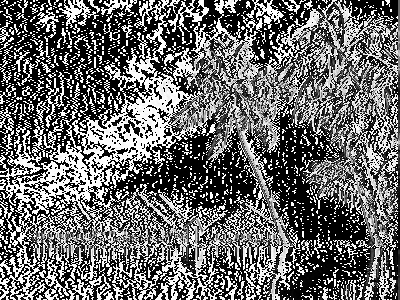
\includegraphics[scale=0.8]{output/p0-4-c-1}}%
	}%
	\caption{Subtracted image (p0-4-c-0) to (p0-1-0) (\textbf{p0-4-c-1})}
	\label{fig:p0-4-c-1}
\end{figure}


The negative values means that the right adjacent pixel was a brighter than the actual pixel, in other words, the intensity of that specific color at that specific pixel is higher than the right pixel next to it.

\newpage

\textbf{Question 5 - Noise} \\

In this question we added some noise to the input image, using a Gaussian function. The Gaussian function normally depends of three variables, however, we are going to vary just the $\sigma$, which is responsible for the range of the generated numbers. \\

\textbf{5-a) }  In this item, we use the generated number to add noise into the green channel of the image. Figure \ref{fig:green-sigma} shows different images obtained with different values of $\sigma$ in the Gaussian function. \\

\begin{figure}[!h]%
	\centering
	\subfloat[$\sigma = 0.5$]{{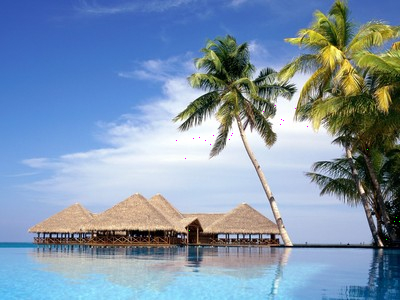
\includegraphics[scale=0.25]{report/sigma-g05.png} }}%
	\quad
	\subfloat[$\sigma = 1$]{{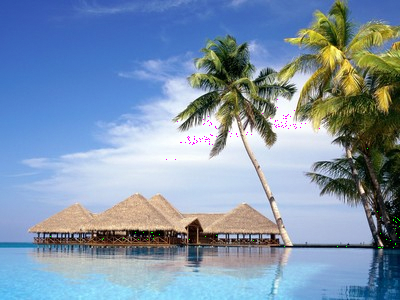
\includegraphics[scale=0.25]{report/sigma-g1} }}%
	\quad
	\subfloat[$\sigma = 5$]{{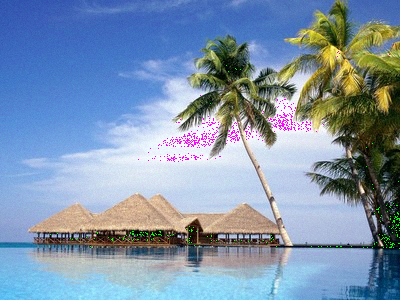
\includegraphics[scale=0.25]{report/sigma-g5} }}%
	\quad
	\subfloat[$\sigma = 10$]{{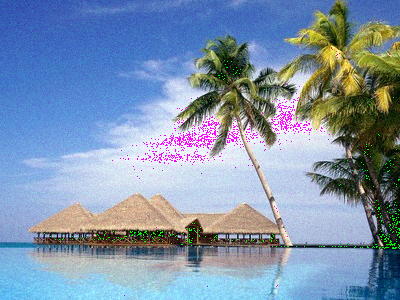
\includegraphics[scale=0.25]{report/sigma-g10} }}%
	\caption{Noise in the green channel from the Gaussian function with different $\sigma$ values}%
	\label{fig:green-sigma}%
\end{figure}

As we can see, the number of noise in the image increases proportionally to $\sigma$. The noise is noticeable once $\sigma = 0.5$, the reason for that is the color of the pixels added. As we are changing the values to the green channel, it makes colors that were white become something similar to pink, which is pretty contrasting between white pixels. We can also see some green points, those come obviously because sometimes the Gaussian adds some intensity to some dark green pixel points.

The final result reported was obtained using a  $\sigma = 10$, and image (\textbf{p0-5-a-0}) shows the result.

\begin{figure}[!h]
	\centering
	{%
		\setlength{\fboxsep}{1pt}%
		\setlength{\fboxrule}{1pt}%
		\fbox{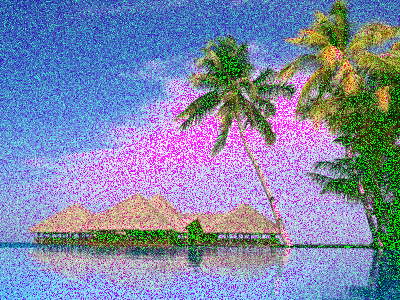
\includegraphics[scale=0.8]{output/p0-5-a-0}}%
	}%
	\caption{Noise added to the green channel (\textbf{p0-5-a-0})}
	\label{fig:p0-5-a-0}
\end{figure}

\newpage

\textbf{5-b) } In this question, we used the same function as before, but now we add the values to the blue channel instead of green. Figure \ref{fig:blue-sigma} shows the result when using different $\sigma$ values. \\

\begin{figure}[!h]%
	\centering
	\subfloat[$\sigma = 0.5$]{{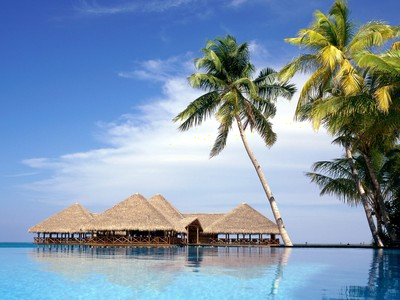
\includegraphics[scale=0.25]{report/sigma-b05.png} }}%
	\quad
	\subfloat[$\sigma = 1$]{{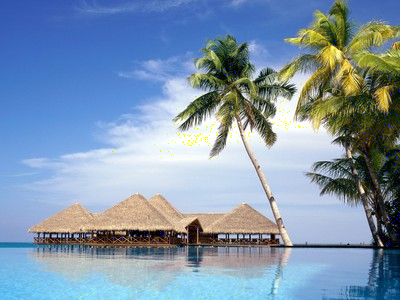
\includegraphics[scale=0.25]{report/sigma-b1} }}%
	\quad
	\subfloat[$\sigma = 5$]{{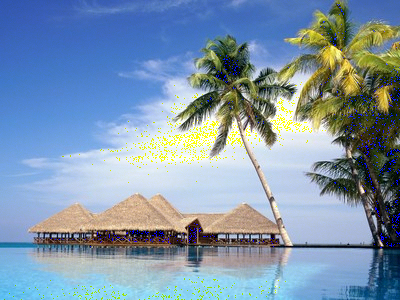
\includegraphics[scale=0.25]{report/sigma-b5} }}%
	\quad
	\subfloat[$\sigma = 10$]{{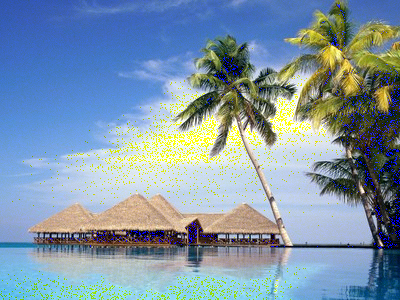
\includegraphics[scale=0.25]{report/sigma-b10} }}%
	\caption{Noise in the blue channel  from the Gaussian function with different $\sigma$ values}%
	\label{fig:blue-sigma}%
\end{figure}

As the other example, the number of noise increases with the $\sigma$ value. However, as we change the blue channel white pixels tend to become a yellow color, which makes the contrast smoother than the pink as seen before.

Image (\textbf{p0-5-b-0}) shows the result submitted in the project, which is using $\sigma = 10$.

\begin{figure}[!h]
	\centering
	{%
		\setlength{\fboxsep}{1pt}%
		\setlength{\fboxrule}{1pt}%
		\fbox{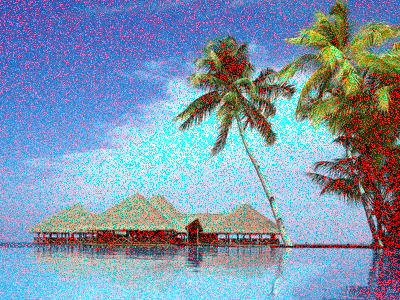
\includegraphics[scale=0.8]{output/p0-5-b-0}}%
	}%
	\caption{p0-5-b-0}
	\label{fig:p0-5-b-0}
\end{figure}


\textbf{5-c) } The image (\textbf{p0-5-b-0}) looks better, the reason is the low level of the contrast that happens between the white and yellow pixels. In image (\textbf{p0-5-a-0}), the high contrast between white and pink makes the image looks too different from the original version.

\end{document}
